\documentclass[tikz,border=10pt]{standalone}
\begin{document}
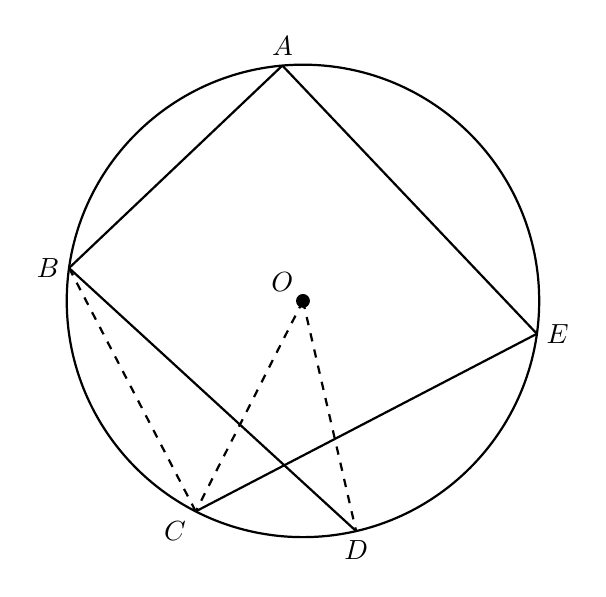
\begin{tikzpicture}[scale=1]
  \coordinate (O) at (0,0);
  \coordinate (A) at (95:3);
  \coordinate (B) at (172:3);
  \coordinate (C) at (243:3);
  \coordinate (D) at (283:3);
  \coordinate (E) at (-8:3);

  \draw[thick] (O) circle (3);
  \fill (O) circle (2.5pt);

  \draw[thick] (A) -- (B);
  \draw[thick] (A) -- (E);
  \draw[thick] (B) -- (D);
  \draw[thick] (C) -- (E);
  \draw[dashed,thick] (B) -- (C);
  \draw[dashed,thick] (O) -- (C);
  \draw[dashed,thick] (O) -- (D);

  \node[above] at (A) {$A$};
  \node[left] at (B) {$B$};
  \node[below left] at (C) {$C$};
  \node[below] at (D) {$D$};
  \node[right] at (E) {$E$};
  \node[above left] at (O) {$O$};
\end{tikzpicture}
\end{document}
